\section{KIỂM TRA THIẾT KẾ}

\subsection{Simulation}
Dựa vào kế hoạch kiểm thử ta tạo một testbench gồm thanh ghi lưu 10000 dữ liệu ảnh từ Test-set MNIST đã được làm phẳng và chuyển thành dạng nhị phân 8-bit và thanh ghi chứa label của từng ảnh. Tạo vòng lặp để lần lượt đưa từng pixel ảnh vào khối DUT để nhận diện đưa qua bộ Checker để so sánh kết quả với label của ảnh và đưa ra console. 
\begin{figure}[H]
    \centering
    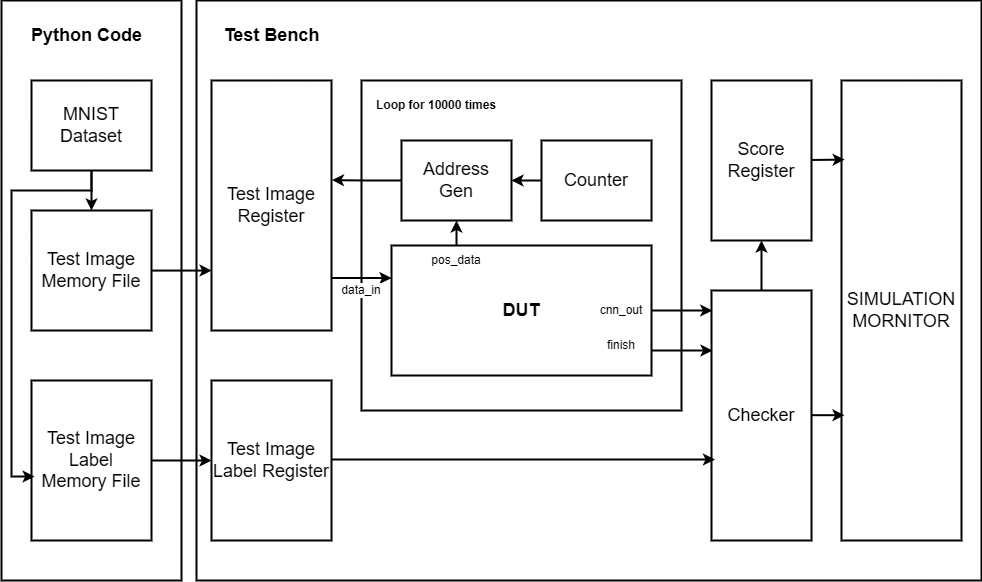
\includegraphics[width=1\linewidth]{Images/cnn_dut_mnist_test.drawio.png}
    \caption{Sơ đồ khối test simulation}
    \label{fig:enter-label}
\end{figure}

Dưới đây là các hình so sánh ngõ ra từng lớp khi chạy tính toán CNN trên FPGA ta thiết kế và model CNN chạy trên Tensorflow. Dữ liệu ảnh từng lớp ngõ ra ta lấy bằng cách dùng tính năng \textit{Export data patterns} để lấy dữ liệu lưu trong khối BSRam và dựa vào bảng memory map \ref{tab:memory_map} để lấy ra ảnh của từng lớp.
\begin{figure}[H]
\centering
    \begin{subfigure}[b]{0.45\linewidth}
        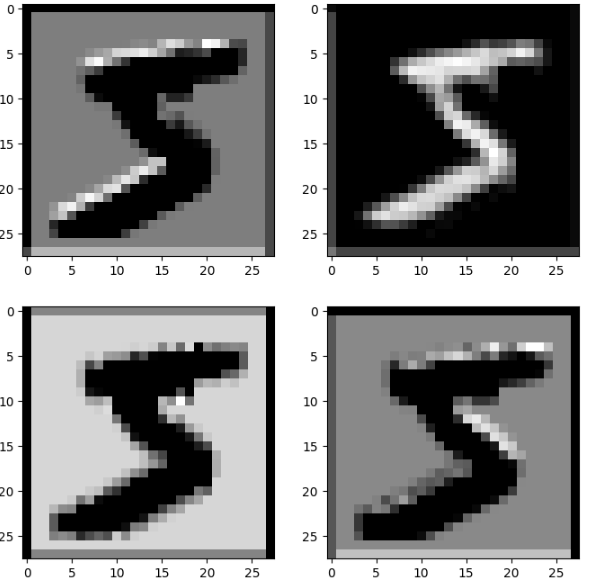
\includegraphics[width=\linewidth]{Images/fpgac1.png}
        \caption{FPGA}
        \label{fig:enter-label}
    \end{subfigure}
    \begin{subfigure}[b]{0.45\linewidth}
        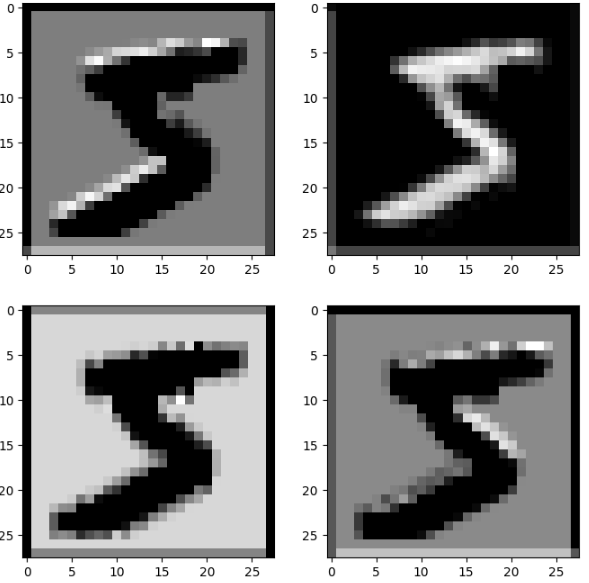
\includegraphics[width=\linewidth]{Images/cnnc1.png}
        \caption{Tensorflow}
        \label{fig:enter-label}
    \end{subfigure}
    \caption{Ảnh ngõ ra lớp Conv1}
    \label{fig:main}
\end{figure}

\begin{figure}[H]
\centering
    \begin{subfigure}[b]{0.45\linewidth}
        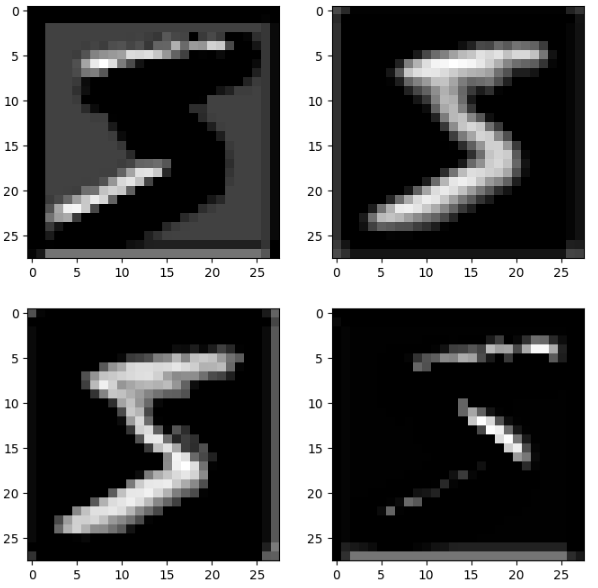
\includegraphics[width=1\linewidth]{Images/fpgac2.png}
        \caption{FPGA}
        \label{fig:enter-label}
    \end{subfigure}
    \begin{subfigure}[b]{0.45\linewidth}
        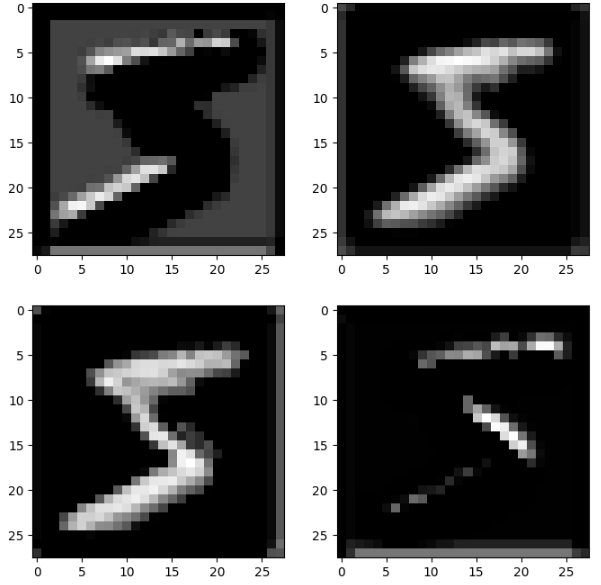
\includegraphics[width=1\linewidth]{Images/cnnc2.png}
        \caption{Tensorflow}
        \label{fig:enter-label}
        \end{subfigure}
    \caption{Ảnh ngõ ra lớp Conv2}
    \label{fig:main}
\end{figure}


\begin{figure}[H]
\centering
    \begin{subfigure}[b]{0.45\linewidth}
        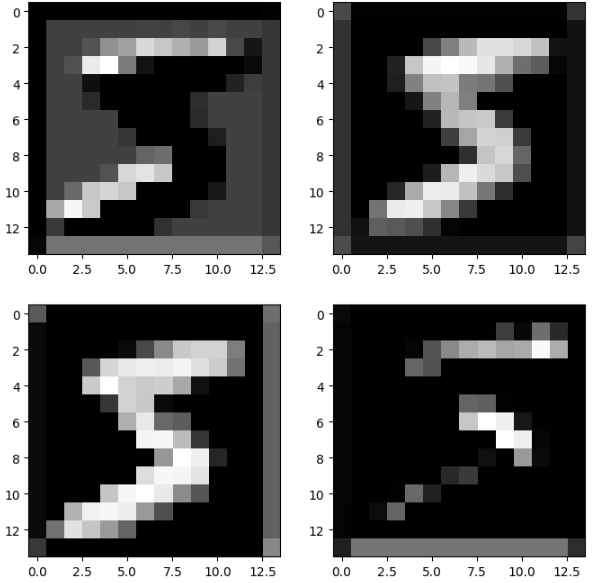
\includegraphics[width=1\linewidth]{Images/fpgam1.png}
        \caption{FPGA}
        \label{fig:enter-label}
    \end{subfigure}
    \begin{subfigure}[b]{0.45\linewidth}
        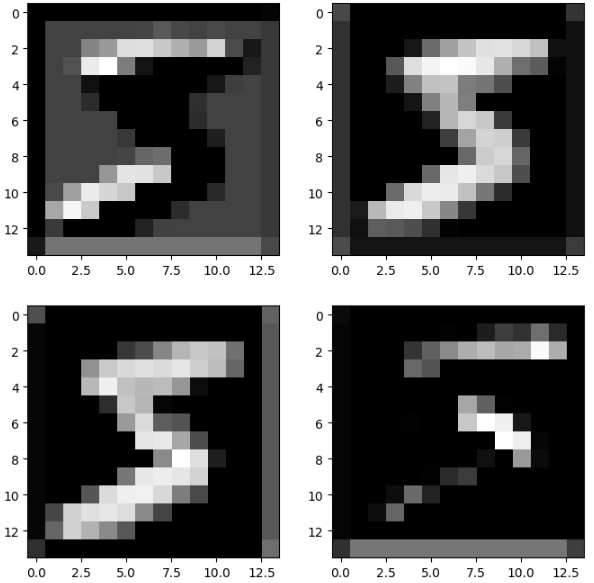
\includegraphics[width=1\linewidth]{Images/cnnm1.png}
        \caption{Tensorflow}
        \label{fig:enter-label}
        \end{subfigure}
    \caption{Ảnh ngõ ra lớp Mpool1}
    \label{fig:main}
\end{figure}

\begin{figure}[H]
\centering
    \begin{subfigure}[b]{0.45\linewidth}
        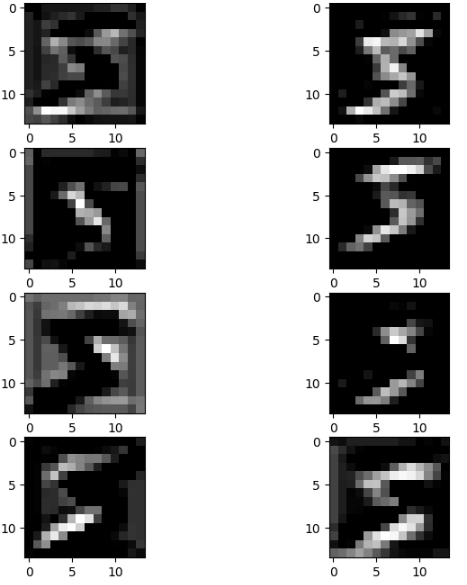
\includegraphics[width=1\linewidth]{Images/fpgac3.png}
        \caption{FPGA}
        \label{fig:enter-label}
    \end{subfigure}
    \begin{subfigure}[b]{0.45\linewidth}
        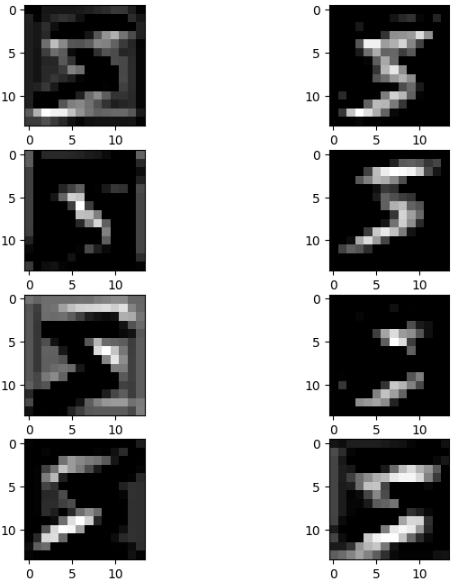
\includegraphics[width=1\linewidth]{Images/cnnc3.png}
        \caption{Tensorflow}
        \label{fig:enter-label}
        \end{subfigure}
    \caption{Ảnh ngõ ra lớp Conv3}
    \label{fig:main}
    \end{figure}


\begin{figure}[H]
\centering
    \begin{subfigure}[b]{0.45\linewidth}
        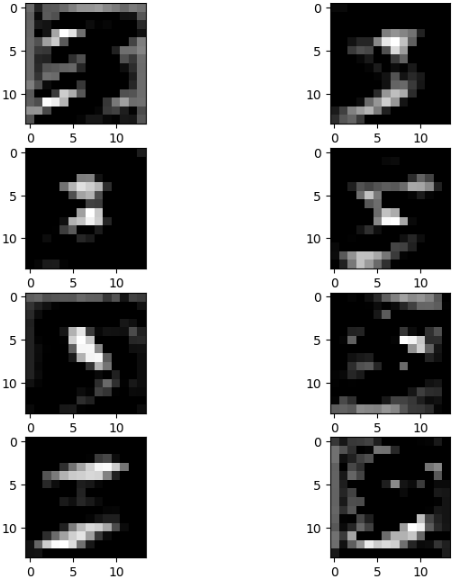
\includegraphics[width=1\linewidth]{Images/fpgac4.png}
        \caption{FPGA}
        \label{fig:enter-label}
    \end{subfigure}
    \begin{subfigure}[b]{0.45\linewidth}
        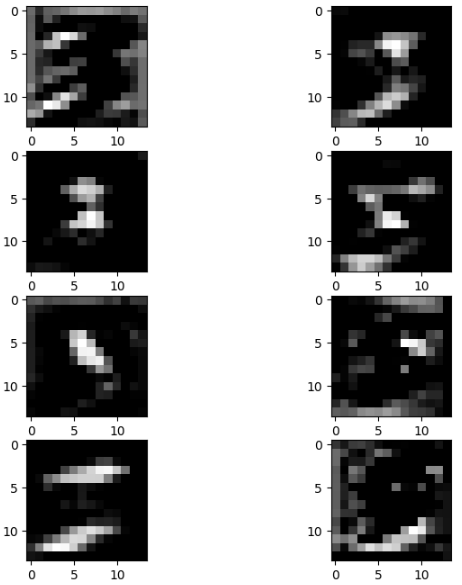
\includegraphics[width=1\linewidth]{Images/cnnc4.png}
        \caption{Tensorflow}
        \label{fig:enter-label}
        \end{subfigure}
    \caption{Ảnh ngõ ra lớp Conv4}
    \label{fig:main}
\end{figure}


\begin{figure}[H]
\centering
    \begin{subfigure}[b]{0.45\linewidth}
        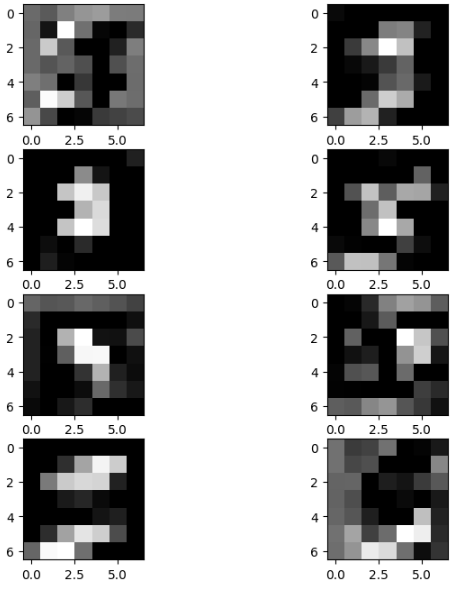
\includegraphics[width=1\linewidth]{Images/fpgam2.png}
        \caption{FPGA}
        \label{fig:enter-label}
    \end{subfigure}
    \begin{subfigure}[b]{0.45\linewidth}
        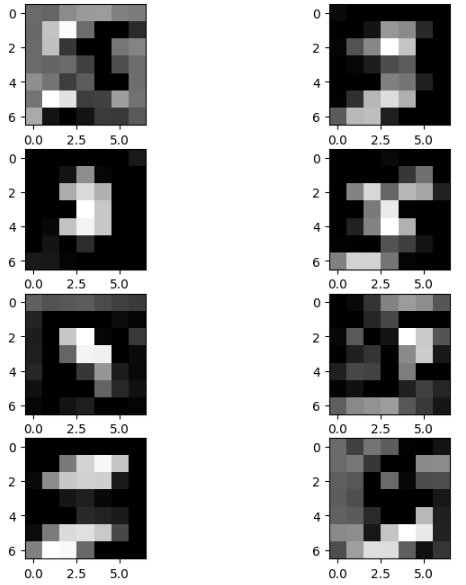
\includegraphics[width=1\linewidth]{Images/cnnm2.png}
        \caption{Tensorflow}
        \label{fig:enter-label}
        \end{subfigure}
    \caption{Ảnh ngõ ra lớp Mpool2}
    \label{fig:main}
\end{figure}


\begin{figure}[H]
\centering
    \begin{subfigure}[b]{0.45\linewidth}
        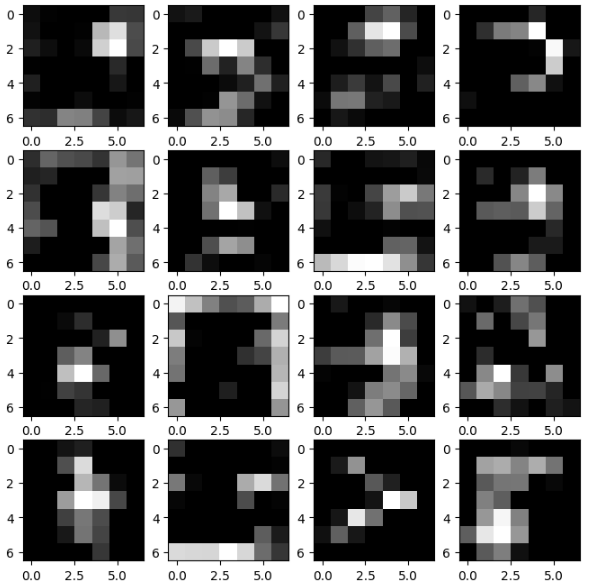
\includegraphics[width=1\linewidth]{Images/fpgac5.png}
        \caption{FPGA}
        \label{fig:enter-label}
    \end{subfigure}
    \begin{subfigure}[b]{0.45\linewidth}
        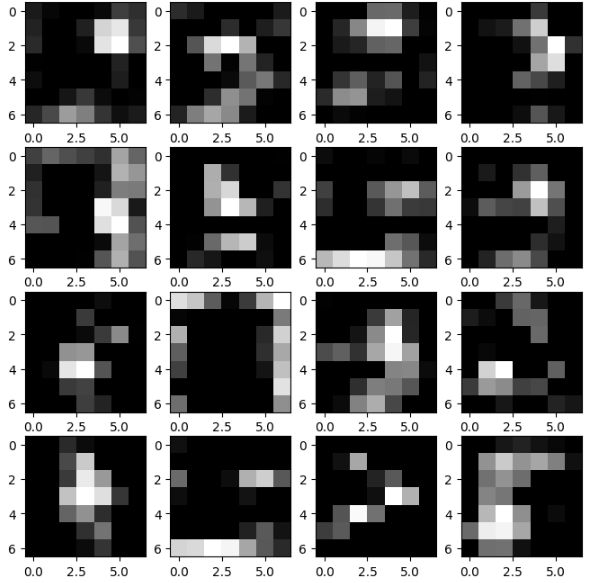
\includegraphics[width=1\linewidth]{Images/cnnc5.png}
        \caption{Tensorflow}
        \label{fig:enter-label}
        \end{subfigure}
    \caption{Ảnh ngõ ra lớp Conv5}
    \label{fig:main}
\end{figure}

\begin{figure}[H]
  \centering
    \begin{subfigure}[b]{\textwidth}
        \centering
        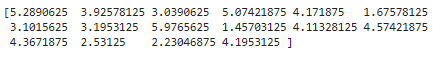
\includegraphics[width=0.75\linewidth]{Images/fpgagm.png}
        \caption{FPGA}
        \label{fig:enter-label}
    \end{subfigure}
    \vspace{1em} % Add vertical spacing
    \begin{subfigure}[b]{\textwidth}
        \centering
        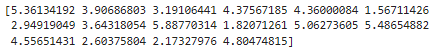
\includegraphics[width=0.75\linewidth]{Images/cnngm.png}
        \caption{Tensorflow}
        \label{fig:enter-label}
    \end{subfigure}
    \caption{Kết quả ngõ ra Global max pooling}
\end{figure}
Ở kết quả ngõ ra Global max pooling có thể thấy kết quả 2 bên có phần chệnh lệch với nhau do các trọng số trên FPGA đã được lượng tử hóa nên sẽ có sai số lượng tử.

\begin{figure}[H]
    \centering
    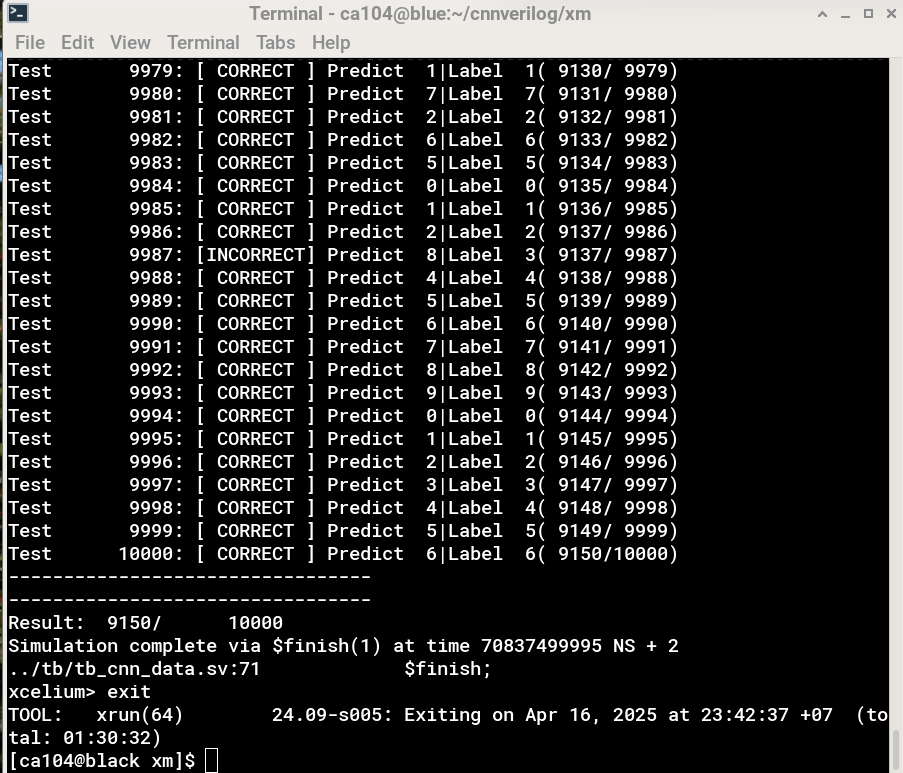
\includegraphics[width=0.75\linewidth]{Images/Screenshot 2025-04-16 192852.png}
    \caption{Giả lập dự đoán tập dữ liệu test MNIST trên Xcelium}
    \label{fig:enter-label}
\end{figure}
Tiến hành test trên bộ dữ liệu Test-set MNIST ta thấy tỉ lệ dự đoán chính xác là 91.5\%, giảm 0.86\% so với mô hình Binary CNN ta tính toán trên máy tính là 92.36\% (Hình \ref{fig:mnisttest}) do ta lượng tử hóa các trọng số về kiểu dữ liệu số fixed-point Q4.8. Thời gian nhận diện 10000 ảnh là $70837499995ns$ với xung clock với chu kì $10ns$ vị chi ta tốn 708375 chu kì clock để nhận diện 1 ảnh. Nếu Module nhận diện số viết tay này sử dụng xung clock 10MHz ta sẽ tốn $\approx71ms$ để xử lí 1 ảnh.

\begin{center}
\begin{table}[H]
\centering
\caption{FPGA-based MNIST Recognition Models Comparison}
\label{tab:mnist_fpga_rotated}
\begin{tabular}{|p{2cm}|p{2cm}|p{2cm}|p{2cm}|p{2cm}|p{2cm}|p{2cm}|}
\hline
\textbf{Model Architecture} & \textbf{Binarized CNN (BNN)} & \textbf{8-bit Quantized CNN} & \textbf{3-Layer MLP} & \textbf{Pruned CNN (Winograd)} & \textbf{Spiking Neural Network} & \textbf{Hybrid CNN-SVM} \\ \hline
\textbf{FPGA Device} & Xilinx Zynq-7020 & Xilinx Virtex-7 & Intel Cyclone V & Xilinx Kintex-7 & Xilinx Spartan-6 & Xilinx Zynq UltraScale \\ \hline
\textbf{LUTs} & 4,500 & 120,000 & 2,300 & 85,000 & 6,200 & 65,000 \\ \hline
\textbf{Clock Cycles} & 30 & 50 & 100 & 20 & 500 & 70 \\ \hline
\textbf{Accuracy (\%)} & 96.4 & 99.1 & 92.0 & 98.5 & 89.7 & 98.8 \\ \hline
\textbf{Freq. (MHz)} & 200 & 150 & 100 & 250 & 50 & 180 \\ \hline
\textbf{Power (W)} & 1.5 & 4.2 & 0.8 & 3.0 & 0.5 & 2.5 \\ \hline
\textbf{Toolchain} & FINN & Vivado HLS & Quartus & Vitis AI & Verilog & PYNQ \\ \hline
\textbf{Year} & 2018 & 2020 & 2017 & 2021 & 2019 & 2022 \\ \hline
\textbf{Remarks} & Binary weights/activations; low power & High DSP usage (256 blocks); pipelined & Minimal resources; no DSP & Winograd transforms; 80\% pruned & Event-driven; ultra-low power & CNN + SVM classifier \\ \hline
\end{tabular}
\end{table}
\end{center}

So sánh model của đồ án này với các model MNIST FPGA khác thì còn nhiều mặt hạn chế như tốc độ xử lý và độ chính xác tuy nhiên cấu trúc của thiết kế đơn giản phù hợp cho việc nghiên cứu cách hoạt động của mạng CNN cũng như FPGA so với các kiến trúc được tạo tự động từ các tool HLS (High-Level Synthesis).

\subsection{Đưa lên kit thực tế}

Để kiểm tra hoạt động của thiết kế ở thực tế ta xây dựng hệ thống đơn giản bằng cách truyền dữ liệu ảnh xám 28x28 cần nhận diện qua UART module nhận diện chữ viết tay như hình \ref{fig:kit}.
\begin{figure}[H]
    \centering
    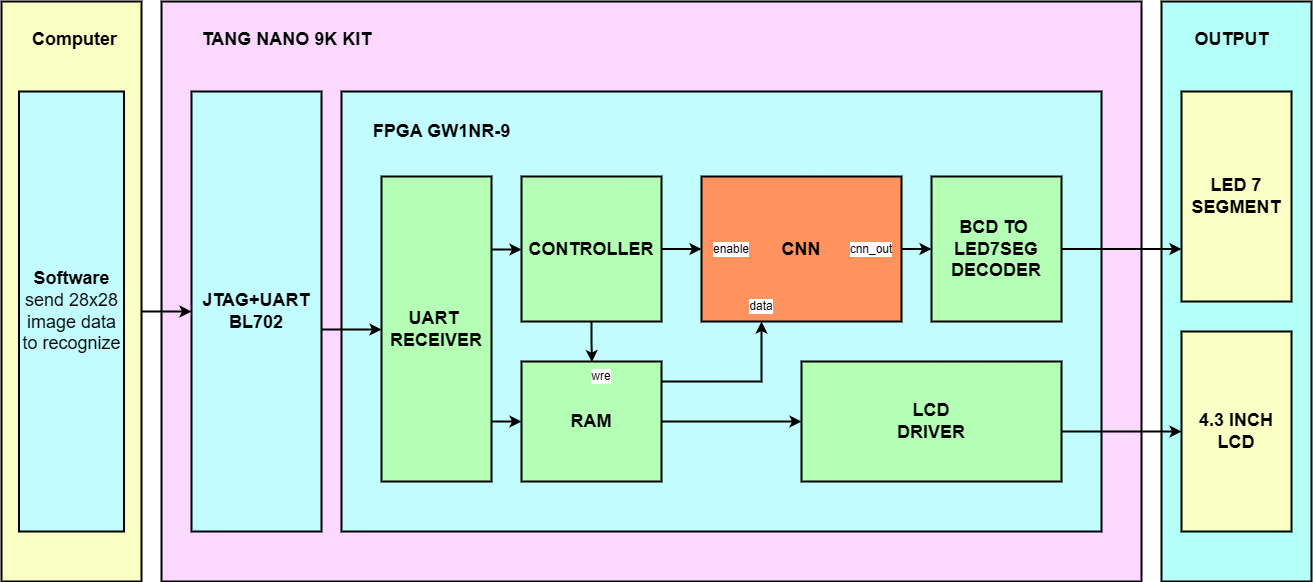
\includegraphics[width=1\linewidth]{Images/cnn_dut_mnist_test-Page-2.drawio.png}
    \caption{Sơ đồ khối hệ thống thực tế}
    \label{fig:kit}
\end{figure}

Với khối UART receiver ta thiết kế như lưu đồ sau.
\begin{figure}[H]
    \centering
    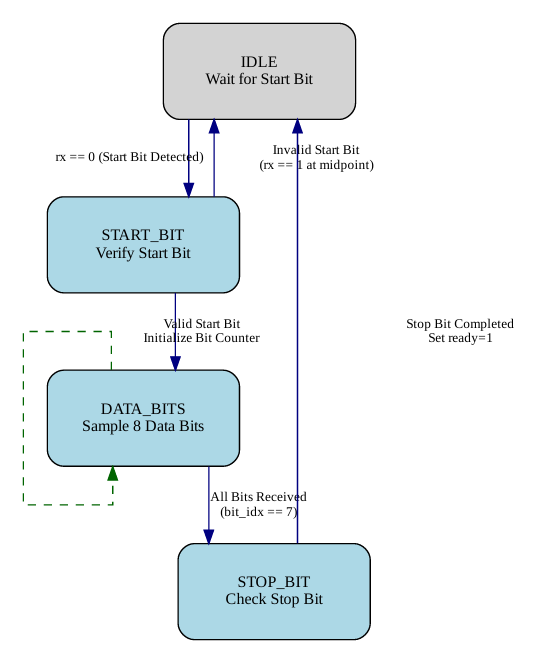
\includegraphics[width=0.5\linewidth]{Images/uartrx.png}
    \caption{UART receiver fsm}
    \label{fig:enter-label}
\end{figure}

Khối controller sẽ nhận các lệnh từ UART bao gồm lệnh load ảnh vào RAM \textit{(nhận kí tự "g")} và lệnh bắt đầu nhân diện số viết tay \textit{(nhận kí tự "d")}.
\begin{figure}[H]
    \centering
    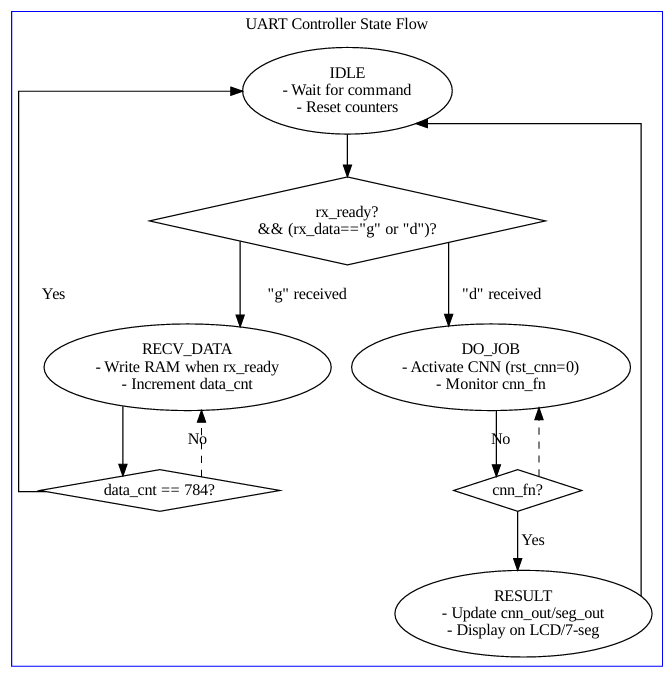
\includegraphics[width=0.6\linewidth]{Images/controller_flow.png}
    \caption{Controller flow chart}
    \label{fig:enter-label}
\end{figure}

Khối LCD Driver có nhiệm vụ đọc dữ liệu ảnh từ RAM và điều khiển các tín hiệu quét ngang và dọc để đưa ảnh lên màn hình.
\begin{figure}[H]
    \centering
    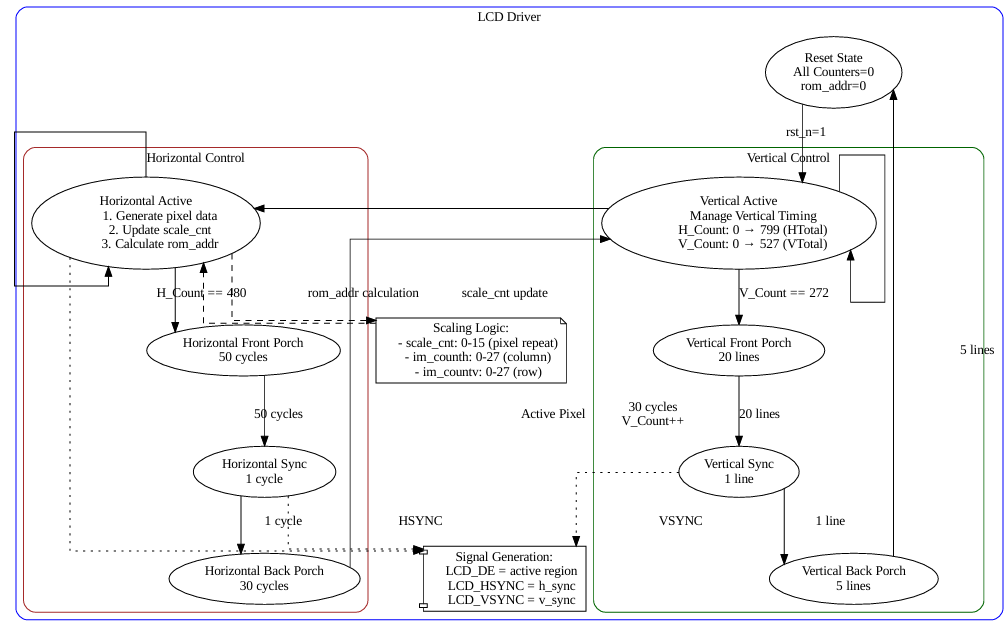
\includegraphics[width=1\linewidth]{Images/lcdriver.png}
    \caption{LCD driver flow chart}
    \label{fig:enter-label}
\end{figure}

Ngoài ra ta cần viết thêm phần mềm đơn giản bằng python sử dung thư viện Tkinter để làm UI và Pyserial để giaop tiếp UART để gửi lệnh và dữ liệu ảnh số viết tay cần nhận diện và có thêm tính năng cho người dùng tự vẽ số viết tay để kiểm tra hoạt động của thiết kế.
\begin{figure}[H]
    \centering
    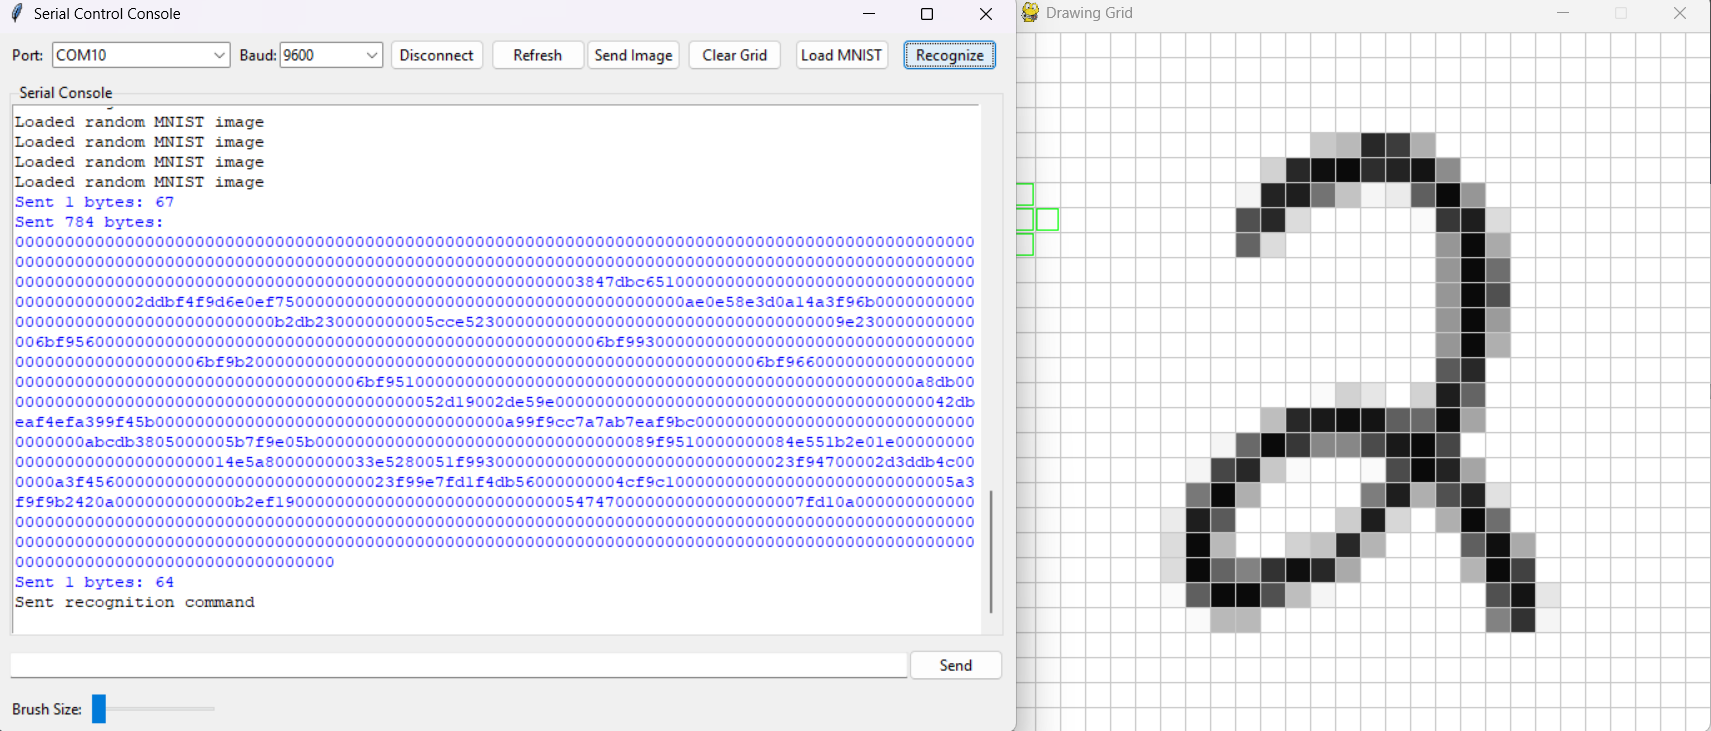
\includegraphics[width=1\linewidth]{Images/sw.png}
    \caption{Giao diện phần mềm}
    \label{fig:sw}
\end{figure}

Gửi hình ảnh số 2 trên phần mềm như hình \ref{fig:sw} và gửi lệnh nhận diện ta có kết quả ngõ ra hiển thị ngõ ra của khối CNN trên led của kit là 0100 và kết quả hiển thị trên led 7 đoạn là 2.
\begin{figure}[H]
    \centering
    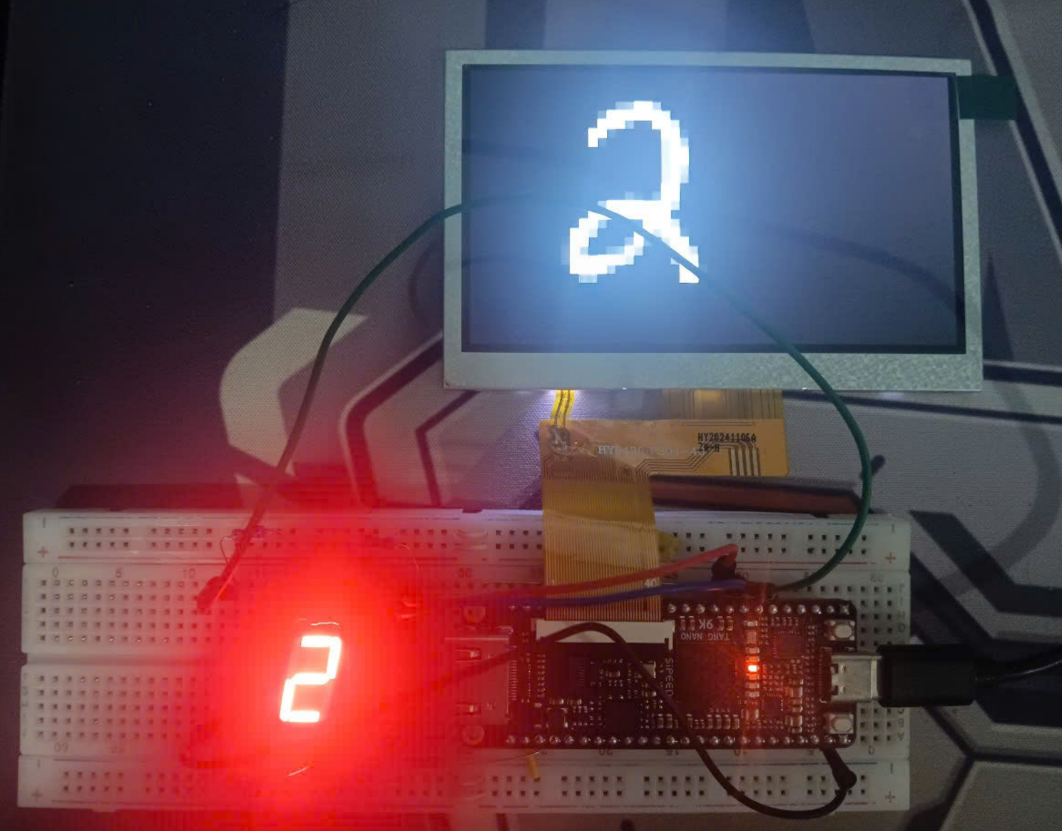
\includegraphics[width=0.75\linewidth]{Images/testr.png}
    \caption{Kết quả nhận diện trên FPGA}
    \label{fig:enter-label}
\end{figure}

Bảng dưới đây là báo cáo tài nguyên mà hệ thống này sử dụng trên kit Tang Nano 9K.
\begin{table}[H]
\centering
\caption{Resource Utilization Summary}
\label{tab:resource_utilization_summary}
\begin{tabular}{l r@{\hspace{1em}}l S[table-format=2.1]}
\toprule
\multirow{2}{*}{\textbf{Resource}} & 
\multicolumn{2}{c}{\textbf{Used/Total}} & 
\multirow{2}{*}{\textbf{Utilization}} \\
& \multicolumn{2}{c}{(units)} & \\
\midrule
Logic & 3305 (1841 LUT, 1446 ALU, 3 RAM16) & / 8640 & 39.0\% \\
Register & 519 & / 6693 & 8.0\% \\
\quad $\bullet$ Register as Latch & 0 & / 6693 & 0.0\% \\
\quad $\bullet$ Register as FF & 519 & / 6693 & 8.0\% \\
BSRAM & 20 & / 26 & 77.0\% \\
\bottomrule
\end{tabular}
\end{table}

Với báo cáo timming với $F_{max}=15.733MHz$ trên kit Tang Nano 9K để cho dễ dàng canh thơi gian cho khung truyền UART ta chọn được tần số 10.8Mhz với baundrate 9600 vì 10.8Mhz chia hết cho 9600 thì UART sẽ truyền dữ liệu tốt nhất.
\begin{figure}[H]
    \centering
    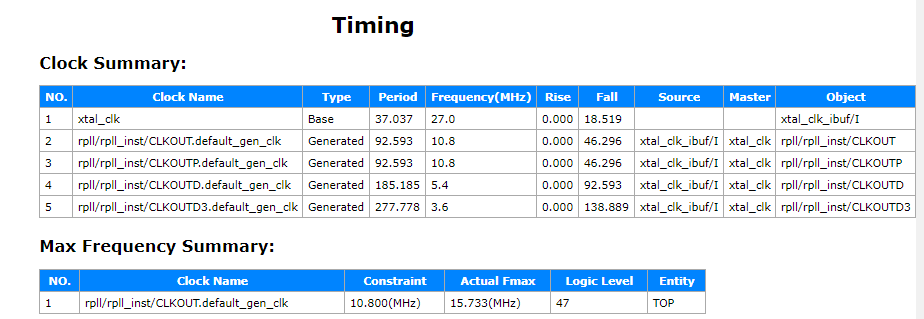
\includegraphics[width=1\linewidth]{Images/timing.png}
    \caption{Báo cáo timming hệ thống}
    \label{fig:enter-label}
\end{figure}
